The scattering of two massive vector bosons (VBS) $VV\to VV$, with $V=W$ or $Z$, is the key process to probe the nature of the electroweak symmetry breaking (EWSB). In the absence of a Standard Model (SM) Higgs boson, the longitudinally polarized VBS amplitude increases as a function of the center-of-mass energy $\sqrt{s}$ and violates unitarity at energies around 1 TeV. The recent discovery of a 125 GeV SM-like Higgs boson at LHC~\cite{AtlasHiggs, CMSHiggs} provides a plausible explanation for the mechanism that unitarizes this process. However, many physics scenarios predict enhancements in the VBS amplitude either from additional resonances, or if the observed SM-like Higgs boson is only partially responsible for the EWSB.\\
At hadron collider VBS can be represented by an interaction of gauge bosons radiated from initial state quarks yielding a final state with two bosons and two jets, in a purely electroweak process. Two classes of processes can generate a $VV + 2 jet$ final state: the first class, that includes also VBS processes, involves only electroweak interactions of order $\alpha_{EW}^{4}$ (\emph{electroweak production}), while the second class involves both strong and electroweak processes of order $\alpha_{S}^{2}\alpha_{EW}^{2}$ (\emph{strong production}). A fiducial region is defined in order to enhance the purity of electroweak $ZZ+2jets$ and remove most of the strong events, which are considered as background in this analysis. This region is a subset of the one we used to measure the inclusive cross section of ZZ processes (see section \ref{sec:results}), in which two $Z$ bosons have a mass between 60 and 120 GeV. In addition to that inclusive region, it requires: at least two jets with an invariant mass ($m_{jj}$) larger than 300 GeV and separated in pseudorapidity by $\Delta\eta_{jj} > 2.4$, the leading(sub-leading) jet with $p_T>100(70)~\mathrm{GeV}$ and the magnitude of the missing transverse energy $E_T < 60~\mathrm{GeV}$. Only one event passing all selection requirements is observed in the data, compared to a SM expectation of 0.14 signal events and 0.47 background events. Figure~\ref{fig:ewk_distr} (left) shows the expected and observed $m_{4\ell}$ distribution after all fiducial region selection criteria are applied, except $\Delta\eta > 2.4$. In this region 4 events are observed and their kinematics is reported in Table~\ref{tab:4ev}. Figure~\ref{fig:ewk_distr} (right) shows the $m_{jj}$ distribution after the whole selection. All three dilepton channels are summed in both plots.
\begin{figure}[hbtp]
  \begin{center}
    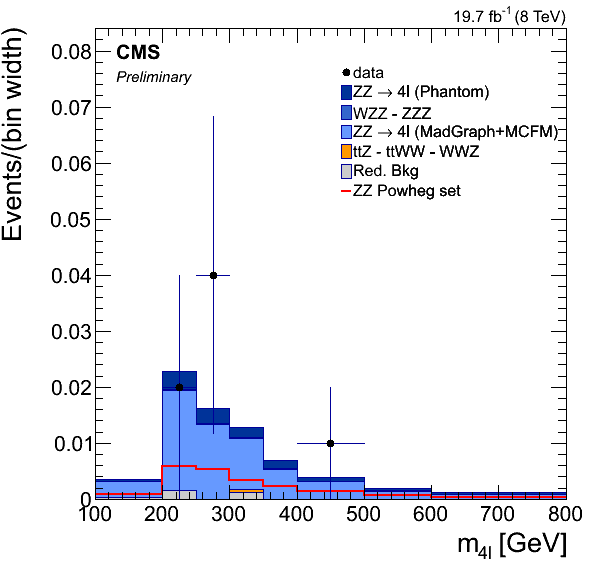
\includegraphics[width=\cmsFigWidth]{Figures/Mass_pt100pt70_met60_mjj200_mad.png}     
    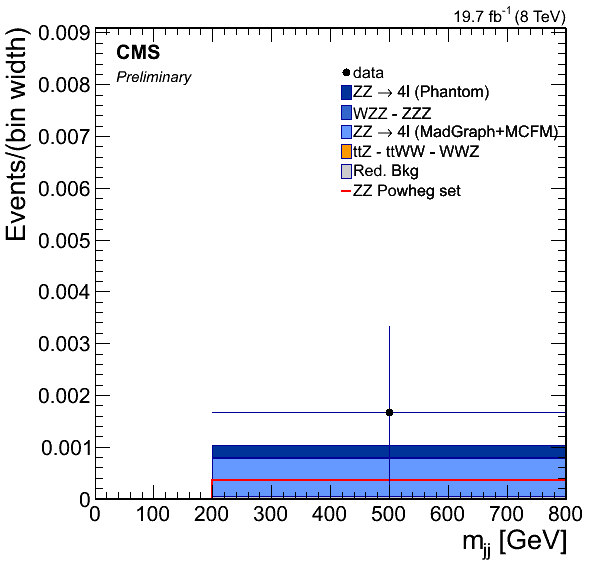
\includegraphics[width=\cmsFigWidth]{Figures/Mjj_pt100pt70_met60_deta24_mad.png}     
       \caption{The $m_{4\ell}$ distribution (left) for events passing the region selections except for the $\Delta\eta_{jj} > 2.4$ selection. The $m_{jj}$ distribution (right) for events passing all the region selections. Points represent the data, the stacked filled histogram represents the predictions for $ZZ$ signal (from \texttt{Phantom}) and background contributions using \texttt{MadGraph} samples to describe $q\bar{q}(qg)\to ZZ\to 4\ell$ processes (while for the stacked histogram outlined in red the \texttt{Powheg} simulation is used).}
    \label{fig:ewk_distr}
  \end{center}
\end{figure}

\begin{table*}[htbH]
\begin{center}
\topcaption{Kinematic values of events observed in the fiducial region without requiring $\Delta\eta_{jj} > 2.4$. \label{tab:4ev}}
\begin{tabular}{lccccc}
\hline Event & $m_{4\ell}$ & $m_{jj}$  & $\Delta\eta_{jj}$ & $p_T^{jet1}$ & $p_T^{jet2}$\\
\hline 1 & 216.6 & 346.6 & 2.64 & 100.3 & 96.47 \\
\hline 2 & 277.7 & 495.2 & 1.20 & 289.5 & 164.2 \\
\hline 3 & 287.2 & 391.5 & 0.97 & 207.5 & 150.4 \\
\hline 4 & 442.5 & 421.9 & 1.59 & 252.3 & 102.9\\
\hline
\end{tabular}
\end{center}
\end{table*}

